\documentclass[11pt]{amsart}
\usepackage{amsmath}
\usepackage{amssymb}
\usepackage{xcolor}
\usepackage{tikz}
\usetikzlibrary{3d}
\usepackage{tikz-3dplot}
\usepackage{pgfplots}

\begin{document}

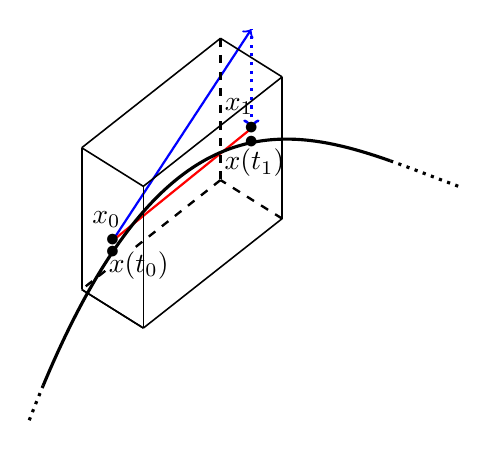
\begin{tikzpicture}[rotate around x=0,rotate around y=45, rotate around z=0,scale=1.8]
%the first box
\draw[->,line width=0.7mm,thick,color=blue] (1,1.58,4.5) -- (2,2.8,4.5);
\draw[<-,line width=0.4mm,dotted,color=blue] (2,2.1,4.5) -- (2,2.8,4.5);
\draw[line width=0.7mm,thick,color=red] (1,1.58,4.5) -- (2,2.1,4.5);

\draw[line width=0.2mm] (1,1.1,5) -- (2,1.6,5);
\draw[line width=0.2mm] (1,1.1,5) -- (1,2.1,5);
\draw[line width=0.2mm] (2,2.6,5) -- (1,2.1,5);
\draw[line width=0.2mm] (2,2.6,5) -- (2,1.6,5);
\draw (1,1.5,4.5) node {$\bullet$};
\draw (1,1.58,4.5) node {$\bullet$};

\draw[line width=0.2mm] (1,2.1,5) -- (1,2.1,4);
\draw[line width=0.2mm] (2,2.6,4) -- (1,2.1,4);
\draw[line width=0.2mm] (2,2.6,4) -- (2,2.6,5);
\draw[line width=0.2mm] (1,1.1,4) -- (1,1.1,5);
\draw (2,2,4.5) node {$\bullet$};
\draw (2,2.1,4.5) node {$\bullet$};


\draw[line width=0.2mm] (1,1.1,4) -- (1,2.1,4);
\draw[line width=0.2mm] (1,1.1,4) -- (1,1.1,5);
\draw[line width=0.3mm,dashed] (2,1.6,5) -- (2,1.6,4);
\draw[line width=0.3mm,dashed] (2,2.6,4) -- (2,1.6,4);
\draw[line width=0.3mm,dashed] (1.17,1.185,4) -- (1,1.1,4);
\draw[line width=0.3mm,dashed] (2,1.6,4) -- (1.36,1.28,4);




\draw[line width=.4mm]
plot[variable=\x,domain=.5:3,samples=73,smooth] 
 (\x,{7/60 *\x^3-23/20 *\x^2+47/15*\x-3/5},4.5);
\draw[line width=.4mm,dotted]
plot[variable=\x,domain=.4:.5,samples=73,smooth] 
 (\x,{7/60 *\x^3-23/20 *\x^2+47/15*\x-3/5},4.5);
\draw[line width=.4mm,dotted]
plot[variable=\x,domain=3:3.5,samples=73,smooth] 
 (\x,{7/60 *\x^3-23/20 *\x^2+47/15*\x-3/5},4.5);

\draw (1, 1.7, 4.4) node {$x_0$};
\draw (1.1, 1.43, 4.7) node {$x(t_0)$};
\draw (2, 2.2, 4.3) node {$x_1$};
\draw (2, 1.87, 4.55) node {$x(t_1)$};

\end{tikzpicture}

\end{document}